\documentclass[a4paper, oneside, openany, dvipsnames, table, 12pt]{article}
\usepackage{../../../Template/AFKstyle}
\usepackage{hyperref}
\usepackage{verbatim} %per commenti di più righe \begin{comment} \end{comment}
\usepackage{amsmath}
\newcommand{\Titolo}{Verbale interno 2020-06-05}

\newcommand{\Gruppo}{TeamAFK}

\newcommand{\Redattori}{}

\newcommand{\Verificatori}{}

\newcommand{\pathimg}{../../../../Template/img/logoAFK.png}

\newcommand{\Approvatore}{}

\newcommand{\Distribuzione}{Prof. Vardanega Tullio \newline Prof. Cardin Riccardo \newline TeamAFK}

\newcommand{\Uso}{Interno}

\newcommand{\NomeProgetto}{"Predire in Grafana"}

\newcommand{\Mail}{gruppoafk15@gmail.com}

\newcommand{\Versionedoc}{1.0.0}

\newcommand{\DescrizioneDoc}{Riassunto dell'incontro del gruppo \textit{TeamAFK} tenutosi il 2020-06-05.}


\makeindex

\begin{document}
\copertina{}

%------------------ COLORI TABELLE 
\definecolor{pari}{RGB}{255, 207, 158} %{HTML}{E1F5FE} %azzurrino
\definecolor{dispari}{HTML}{FAFAFA} %bianco/grigetto 

%definizione colori per tabelle (tranne copertina)
\definecolor{redafk}{RGB}{255, 133, 51}
\definecolor{grey2}{RGB}{204, 204, 204}
\definecolor{greyRowafk}{RGB}{234, 234, 234}
\definecolor{lastrowcolor}{RGB}{176, 196, 222} %steel blue %{255,165,0} orange %{RGB}{255, 207, 158}
\rowcolors{2}{pari}{dispari}
\renewcommand{\arraystretch}{1.5}

%------------------

\newpage
\section*{Registro delle modifiche}
{
	\centering
	\begin{longtable}{ c c  C{4cm}  C{4cm}  C{3cm} }
		\rowcolor{redafk}
		\textcolor{white}{\textbf{Versione}} & \textcolor{white}{\textbf{Data}} & \textcolor{white}{\textbf{Descrizione}} & \textcolor{white}{\textbf{Nominativo}} & \textcolor{white}{\textbf{Ruolo}}\\		
		2.1.1 & 2020-05-27 & Aggiunta incrementi \S 6.2. Verificato il documento. & &\adm{} \newline \ver{} \\
		2.1.0 & 2020-05-26 & Refactoring \S 4.1 e \S 4.3. Apportate modifiche normative al \textit{Registro delle Modifiche}. Verificato il documento. & Davide Zilio \newline Victor Dutca & \adm{} \newline \ver{} \\
		2.0.0 & 2020-05-10 & Approvazione del documento per la RP. & Davide Zilio &\RdP{} \\
		1.1.0 & 2020-05-08 & Stesura \S 6.2. Verificato il documento. & Simone Meneghin \newline Alessandro Canesso &\adm{} \newline \ver{}\\
		1.0.2 & 2020-05-06 & Ampliamento \S 2. Verificato il documento. & Victor Dutca \newline Alessandro Canesso &\Res{} \newline \ver{}\\
		1.0.1 & 2020-04-30 & Correzioni e stesura \S 2.1. Verificato il documento. & Simone Meneghin \newline Alessandro Canesso &\Res{} \newline \ver{}\\
		1.0.0 & 2020-04-12 & Approvazione del documento per la RR. & Victor Dutca &\RdP{} \\
		0.7.0 & 2020-03-10 & Stesura \S B. Verificato il documento. & Alessandro Canesso \newline Olivier Utshudi &\Res{} \newline \ver{}\\
		0.6.0 & 2020-03-10 & Stesura \S 6. Verificato il documento. & Alessandro Canesso \newline Olivier Utshudi &\Res{} \newline \ver{}\\
		0.5.0 & 2020-03-06 & Stesura \S 5. Verificato il documento.  & Fouad Farid \newline Olivier Utshudi &\Res{} \newline \ver{}\\
		0.4.0 & 2020-04-04 & Stesura \S 4. Verificato il documento. & Simone Federico Bergamin \newline Simone Meneghin &\adm{} \newline \ver{}\\	
		0.3.0 & 2020-04-03 & Stesura \S 3. Verificato il documento.  & Simone Federico Bergamin \newline Olivier Utshudi &\adm{} \newline \ver{}\\	
		0.2.0 & 2020-03-30 & Stesura \S 2. Verificato il documento.  & Alessandro Canesso \newline Simone Meneghin &\Res{} \newline \ver{}\\	
		0.1.0 & 2020-03-30 & Stesura \S 1. Verificato il documento. & Alessandro Canesso \newline Simone Meneghin &\Res{} \newline \ver{}\\		
	\end{longtable}
} 


%Didascalia tabelle/immagini (prendono come riferimento la subsection)
\counterwithin{table}{subsection}
\newpage

%indice, indice figure e indice tabelle
\tableofcontents
\newpage

\listoftables
\newpage

\listoffigures
\newpage

\section{Introduzione}

\subsection{Scopo del documento}
Il seguente documento ha il compito di stabilire le regole che il team di sviluppo intende seguire in ogni attività di progetto, così da omologare il materiale prodotto.
I fornitori intendono adottare un approccio incrementale\glo, affinché lo sviluppo del prodotto si basi su decisioni prese di comune accordo. Perciò ogni componente del team deve far riferimento a questo documento per garantire la coesione e uniformità delle scelte prese.

\subsection{Scopo del prodotto}
Il capitolato {C4}\glo illustra il prodotto da fornire. Tale prodotto consiste in tool di addestramento ed un plugin\glo di Grafana\glo che prenderà il nome \textit{Predire in Grafana}. Entrambi gli applicativi verranno scritti in linguaggio JavaScript\glo. Il primo avrà il compito di produrre un file di estensione JSON\glo basato su dati di addestramento\glo. Il secondo invece si occuperà di leggere il file creato, effettuare previsioni basandosi su di esso e rendere disponibili al sistema i risultati ottenuti, in modo da poterli visualizzare in grafici e dashboard.
\subsection{Glossario}
Per evitare ambiguità nei documenti formali, viene fornito il documento \textit{Glossario\_v2.0.0}, contenente tutti i termini considerati di difficile comprensione. Perciò nella documentazione fornita ogni vocabolo contenuto in \textit{Glossario\_v2.0.0} è contrassegnato dalla lettera \textit{G} a pedice.
\subsection{Riferimenti}
\subsubsection{Riferimenti normativi}
\begin{itemize}
	\item \textbf{Capitolato d'appalto C4 - Predire in Grafana}: \\
	\url{https://www.math.unipd.it/~tullio/IS-1/2019/Progetto/C4.pdf}.	
\end{itemize}
\subsubsection{Riferimenti informativi}
\begin{itemize}
	\item \textbf{Change Management Process}: \\
	\href{https://www.blog-management.it/2018/04/10/change-management-project-management/}{https://www.blog-management.it/change-management-project-management}\\
	\href{https://www.digital4.biz/hr/hr-transformation/digital-transformation-e-change-management-vanno-avanti-di-pari-passo/}{https://www.digital4.biz/hr/hr-transformation/};
	\item \textbf{The three P's of Software Engineering}: \\
	\url{http://dwaynephillips.net/CutterPapers/ppp/ppp.htm}
	\item \textbf{Software Engineering - Ian Sommerville - 10th Edition}
	\item \textbf{Slide L05 del corso Ingegneria del Software - Ciclo di vita del software}: \\
	\url{https://www.math.unipd.it/~tullio/IS-1/2019/Dispense/L05.pdf};
	\item \textbf{Slide L06 del corso Ingegneria del Software - Gestione di Progetto}: \\
	\url{https://www.math.unipd.it/~tullio/IS-1/2019/Dispense/L06.pdf};	
	\item \textbf{Slide L12 del corso Ingegneria del Software - Qualità di Prodotto}: \\
	\url{https://www.math.unipd.it/~tullio/IS-1/2019/Dispense/L12.pdf};
	\item \textbf{Slide L13 del corso Ingegneria del Software - Qualità di Processo}: \\
	\url{https://www.math.unipd.it/~tullio/IS-1/2019/Dispense/L13.pdf};
\end{itemize}
\pagebreak

\section{Qualità di processo}
\subsection{Scopo}
Al fine di garantire la qualità del prodotto è necessario perseguire in primis la qualità dei processi che la definiscono. Si è deciso dunque di aderire, per quanto possibile, allo standard \textbf{ISO/IEC 15504}\footnote{ISO/IEC 15504: insieme di documenti di standard tecnici relativi ai processi di sviluppo del software e relative funzioni di business e, in particolare, alla loro valutazione.} denominato SPICE\glo: quest'ultimo permette di valutare il livello di maturità e capacità\glo (capability) dei processi, al fine di apportare modifiche migliorative. 
\begin{comment}
Eliminato la subsection PDCA
\end{comment}
\subsection{Obiettivi}
Sono fissati inoltre i seguenti obiettivi: \begin{itemize}
\item rispetto di tempi e costi descritti nel \textit{Piano\_di\_Progetto\_v2.0.0};
\item continuo miglioramento dei processi;
\item misurabilità dello stato dei processi.
\end{itemize}
\subsection{Metriche}
Per misurare la qualità, sono state scelte delle specifiche metriche che monitorano lo stato dei processi del progetto analizzando l'uso che essi fanno di tempo e denaro. Sono particolarmente utili per il \textit{Responsabile}, che può quindi decidere di apportare modifiche alla pianificazione quando necessario.\\
Ogni metrica conterrà:
\begin{itemize}
\item \textbf{Nome};
\item \textbf{Descrizione};
\item \textbf{Parametri}: range di valori su cui confrontare le misure ottenute. Sono definiti i seguenti intervalli: \begin{itemize}
\item \textbf{Accettabile}: intervallo in cui il valore misurato viene considerato sufficiente, seppur migliorabile;
\item \textbf{Ottimale}: intervallo in cui il valore misurato viene ritenuto ottimo.
\end{itemize}
Tali intervalli possono essere: \begin{itemize}
\item \textbf{Aperti}, se gli estremi non sono compresi. Esempio: (a, b) = $a < x < b$; 
\item \textbf{Chiusi}, se gli estremi sono compresi. Esempio: [a, b] = $a \leq x \leq b$;
\item \textbf{Limitati}, se gli estremi sono numeri finiti;
\item \textbf{Illimitati}, se almeno uno degli estremi è infinito.
\end{itemize}
\end{itemize}
\textbf{Attenzione}: in questo documento \textbf{non} saranno trattati la descrizione e gli strumenti per il calcolo delle metriche, reperibili invece nelle \textit{Norme\_di\_Progetto\_v2.0.0}.

\subsubsection{MP01 - Schedule Variance} 
La Schedule Variance indica se una certa attività o processo è in anticipo, in pari, o in ritardo rispetto alla data di scadenza prevista. \\ \\ 
\textbf{Parametri adottati:} 
\begin{itemize}
\item range accettabile: ($ -\infty $, 2];
\item range ottimale: ($ -\infty $, 0].
\end{itemize}

\subsubsection{MP02 - Budget Variance} 
Permette di controllare i costi sostenuti alla data corrente rispetto al budget preventivato in termini percentuali. \\ \\ 
\textbf{Parametri adottati:}  
\begin{itemize}
\item range accettabile: [$-15\%$, $0\%$); 
\item range ottimale: $ \geq 0\%$.
\end{itemize}

\subsubsection{MP03 - Produttività} 
Rappresenta la produttività media delle risorse impiegate, cioè delle persone coinvolte, nelle diverse fasi del progetto. \\ \\ 
\textbf{Parametri adottati:} 
\begin{itemize}
	\item range accettabile: [50, 100];
	\item range ottimale: $ > 100$.
\end{itemize}

\subsection{Riepilogo metriche}
\begin{longtable}{C{2cm} C{4cm} C{5cm}}
\rowcolor{white}
\caption{Tabella riepilogativa delle metriche per la qualità dei processi}\\
\rowcolor{redafk}
	\textcolor{white}{\textbf{Codice}} &
	\textcolor{white}{\textbf{Nome}} &
	\textcolor{white}{\textbf{Range}} \\
		\endfirsthead
		\rowcolor{white}\caption[]{(continua)} \\
		\rowcolor{redafk}
\textcolor{white}{\textbf{Codice}} &
\textcolor{white}{\textbf{Nome}} &
\textcolor{white}{\textbf{Range}} \\
		\endhead
			MP01 &
Schedule Variance &
\textbf{Accettabile}: (0, 5]
\textbf{Ottimale}: ($ -\infty $, 0] \\
MP02 &
Budget Variance &
\textbf{Accettabile}: [$-15\%$, $0\%$)
\textbf{Ottimale}: $ \geq $ 0 \\
MP03 &
Produttività &
\textbf{Accettabile}: [50, 100]
\textbf{Ottimale}: $ > 100$ \\	
\end{longtable}
\pagebreak

\section{Qualifica di prodotto}
\subsection{Scopo}
Per stabilire la Qualità di prodotto, il team di Quality Management\glo adotta come standard di riferimento \textbf{ISO/IEC 9126} per stabilire il modello della qualità del software. Per decretare il raggiungimento di un determinato obiettivo di qualità, ogni voce trattata è accompagnata da un apposito parametro.
\subsection{Obiettivi}
Gli obiettivi di qualità che il team di Quality Management vuole raggiungere sono:
\begin{itemize}
\item affidabilità;
\item usabilità.
\end{itemize}
\subsection{Metriche della documentazione}
In relazione agli obiettivi prestabiliti, il team adotta i diversi strumenti per misurare la qualità del prodotto, riportati di seguito.
\subsubsection{MD01 - Indice di Gulpease}
L'Indice di Gulpease registra la leggibilità di un documento. \\ \\ 
\textbf{Parametri adottati:} 
\begin{itemize}
\item range accettabile: [40, 60);
\item range ottimale: [60, 100].
\end{itemize}
\subsection{Metriche del codice sorgente}
\subsubsection{MS01 - Linee di Codice}
È la metrica che registra la dimensione di tutto il codice sorgente di un metodo.\\ \\
\textbf{Parametri adottati:}
\begin{itemize}
\item range accettabile: (10, 20];
\item range ottimale: [1, 10].
\end{itemize}
\subsubsection{MS02 - Numero dei Metodi}
Questa metrica conteggia il numero di metodi presenti nella classe di un oggetto.\\ \\ 
\textbf{Parametri adottati:} 
\begin{itemize}
\item range accettabile: (8, 15];
\item range ottimale: [0, 8].
\end{itemize}
\subsubsection{MS03 - Numero di Parametri}
Questo strumento tiene conto del numero di parametri formali di un metodo.\\ \\ 
\textbf{Parametri adottati:} 
\begin{itemize}
\item range accettabile: (3, 6];
\item range ottimale: [0, 3].
\end{itemize}
\subsubsection{MS04 - Commenti per Linee di Codice}
È il rapporto tra le righe di commento e il codice effettivo.\\ \\ 
\textbf{Parametri adottati:} 
\begin{itemize}
\item range accettabile: [0.05, 0.10);
\item range ottimale: [0.10, 0.20].
\end{itemize}
\subsubsection{MS05 - Code Coverage}
È la metrica con il compito di misurare l'indice di copertura del codice da parte dei test in termini percentuali.\\ \\ 
\textbf{Parametri adottati:} 
\begin{itemize}
\item range accettabile: [70, 80)\%;
\item range ottimale: [80, 100]\%.
\end{itemize}
Seppur l'obiettivo del team di sviluppo sia quello di avere una Code Coverage del 100\%, tale traguardo potrebbe non essere raggiunto in quanto comporterebbe un aumento dei costi di progetto che risulterebbero troppo elevati.
\pagebreak

\section{Specifica dei test}
Per verificare la qualità del prodotto software, il gruppo fornitore ha deciso di adottare il \textbf{Modello di Sviluppo a V}\glo, sviluppando così una serie di test. Questi hanno lo scopo di controllare che tutte le unità di cui è composto il sistema siano state implementate correttamente, rispettando tutti gli aspetti del progetto.
Per semplificare la loro consultazione i test saranno suddivisi in categorie, per mezzo di tabelle, mostrando l'output prodotto e sottolineando se è un risultato atteso o non atteso.
\subsection{Stato dei test}
Per definire lo stato dei test, si usano le seguenti sigle:
\begin{itemize}
\item \textbf{I}: test implementato;
\item \textbf{NI}: test non implementato.
\end{itemize}

\begin{longtable}{C{2.5cm} C{2.5cm} L{8cm} C{2cm}}
\rowcolor{white}\caption{Tabella dei test} \\
		\rowcolor{redafk}
\textcolor{white}{\textbf{Codice}} &
\textcolor{white}{\textbf{Caso d'uso}} &
\textcolor{white}{\textbf{Descrizione}} &
\textcolor{white}{\textbf{Esito}} \\
		\endfirsthead
		\rowcolor{white}\caption[]{(continua)} \\
		\rowcolor{redafk}
\textcolor{white}{\textbf{Requisito}} &
\textcolor{white}{\textbf{Caso d'uso}} &
\textcolor{white}{\textbf{Descrizione}} &
\textcolor{white}{\textbf{Esito}} \\
		\endhead
%-------------------------------------------- Simo		
TSOF1 & UC1 &
L'utente  deve poter creare il file JSON\glo contenente il/i predittore/i\glo. \newline
All'utente viene chiesto di:
\begin{itemize}
	\item cliccare il pulsante “Carica Dati di Addestramento”;
	\item scegliere i dati di addestramento\glo da caricare;
	\item selezionare l’algoritmo di previsione\glo;
	\item conferma delle operazioni;
	\item salvataggio file JSON contenente i predittori.
\end{itemize} & I \\

TSOF1.1 & UC1.1 &
L'utente  deve poter caricare i dati di addestramento. \newline All'utente viene chiesto di:
\begin{itemize}
 	\item cliccare il pulsante "Carica Dati di Addestramento";
 	\item verificare che si apra la finestra che visualizza il file system\glo.
\end{itemize} & I	\\


TSOF1.2 & UC1.2 &
L'utente  deve poter scegliere i dati di addestramento. \newline All'utente viene chiesto di:
\begin{itemize}
 	\item verificare che dalla finestra di dialogo siano visibili solo file CSV\glo;
	\item selezionare i dati di addestramento.
\end{itemize} 
& I \\
 
TSOF1.3 & UC1.3 & 
L'utente deve poter scegliere l'algoritmo di predizione. \newline All'utente viene chiesto di:
\begin{itemize}
	\item cliccare sulla Combo Box\glo con etichetta "Seleziona Algoritmo";
	\item scegliere uno degli algoritmi proposti (RL o SVM).
\end{itemize} & I \\
 
TSOF1.4 & UC1.4 & 
L'utente deve poter confermare la scelta dell'algoritmo. \newline All'utente viene chiesto di:
\begin{itemize}
	\item cliccare sul pulsante "Conferma".
\end{itemize} & I \\

TSOF1.4.1 & UC9 & 
L'utente deve poter visualizzare un messaggio d'errore se la scelta dell'algoritmo non è compatibile con i dati di addestramento. \newline All'utente viene chiesto di:
\begin{itemize}
	\item verificare la visualizzazione dell'errore;
	\item verificare di essere rimandati al TSOF1.2.
\end{itemize} & I \\

TSOF2 & UC2 &
L'utente  deve poter caricare il file JSON nel plug-in. \newline All'utente viene chiesto di:
\begin{itemize}
	\item cliccare il pulsante per caricare il file JSON;
	\item selezionare il file JSON;
	\item confermare il caricamento del file.
\end{itemize} & I	\\


TSOF2.1 & UC2.1 &
L'utente  deve poter caricare il file JSON. \newline All'utente viene chiesto di:
\begin{itemize}
	\item cliccare su "Carica JSON";
	\item verificare la visualizzazione della finestra di selezione file.
\end{itemize} & I	\\

TSOF2.1.1 & UC10 &
L'utente  deve poter visualizzare il messaggio di alert\glo del caricamento già avvenuto e caricare nuovamente il file. \newline All'utente viene chiesto di:
\begin{itemize}
	\item visualizzare il messaggio di alert "File JSON già caricato";
	\item cliccare su "Conferma" per sovrascrivere il file.
\end{itemize} & NI	\\

TSOF2.1.2 & UC10 &
L'utente  deve poter visualizzare il messaggio di alert del caricamento già avvenuto e annullare il caricamento. \newline All'utente viene chiesto di:
\begin{itemize}
	\item visualizzare il messaggio di alert "File JSON già caricato";
	\item cliccare su "Annulla" per tornare alla sezione di caricamento.
\end{itemize} & NI	\\

TSOF2.2 & UC2.2 &
L'utente  deve poter selezionare il file JSON. \newline All'utente viene chiesto di:
\begin{itemize}
	\item verificare che siano visibili solo file JSON;
	\item selezionare il file dalla finestra di dialogo.
\end{itemize} & I	\\

TSOF2.3 & UC2.3 &
L'utente  deve poter confermare il caricamento del file. \newline All'utente viene chiesto di:
\begin{itemize}
	\item cliccare sul pulsante "Conferma".
\end{itemize} & I	\\


TSOF2.3.1 & UC11 &
L'utente  deve poter visualizzare un messaggio d'errore in caso di problemi con il caricamento. \newline All'utente viene chiesto di:
\begin{itemize}
	\item visualizzare il messaggio d'errore "Struttura del file JSON non Supportata";
	\item cliccare il pulsante "Conferma";
	\item verificare di essere ritornato alla selezione del file.
\end{itemize} & NI	\\

TSOF2.3.2 & UC17 &
L'utente  deve poter visualizzare un messaggio di notifica di caricamento avvenuto con successo. \newline All'utente viene chiesto di:
\begin{itemize}
	\item visualizzare il messaggio di notifica "Avvenuto Successo Caricamento File JSON";
	\item cliccare il pulsante "Continua".
\end{itemize} & NI	\\
%-------------------------------------------- Olly
TSOF3 & 
UC3 &
L'utente  deve poter collegare un predittore ad un flusso. In particolare l'utente deve:
\begin{itemize}
	\item poter visualizzare la schermata di collegamento;
	\item poter selezionale il server di Grafana a cui collegarsi.
\end{itemize} &
NI \\ 

TSOF3.1 &
UC3.1 &
L'utente  deve poter selezionare il Database\glo. All'utente viene chiesto di:
\begin{itemize}
	\item verificare l'effettiva connessione al server;
	\item visualizzare la lista di Database disponibili;
	\item verificare di poter selezionare il Database desiderato.
\end{itemize}&
NI \\

TSOF3.2 &
UC3.2 &
L'utente  deve poter selezionare almeno un flusso di dati. All'utente viene chiesto di:
\begin{itemize}
	\item visualizzare le tabelle del Database;
	\item verificare di poter selezionare il flusso desiderato;
	\item verificare di poter utilizzare i dati del flusso selezionato.
\end{itemize}&
NI \\

TSOF3.3 &
UC3.3 &
L'utente  deve poter selezionare il predittore da associare al flusso. All'utente viene chiesto di:
\begin{itemize}
	\item visualizzare l'elenco dei predittori;
	\item verificare di poter selezionare il/i predittore/i desiderato/i;
	\item verificare la buona riuscita del collegamento.
\end{itemize}&
NI \\

TSOF3.4 &
UC3.4 &
L'utente  deve poter selezionare un nodo\glo del flusso. All'utente viene chiesto di:
\begin{itemize}
	\item verificare di poter selezionare il nodo desiderato;
	\item verificare di aver a disposizione il nodo desiderato.
\end{itemize}&
NI \\

TSOF3.5 &
UC3.5 &
L'utente  deve poter stabilire una o più soglie\glo al predittore. All'utente viene chiesto di:
\begin{itemize}
	\item  verificare se la funzionalità è disponibile;
	\item verificare se la soglia impostata è effettivamente quella desiderata.
\end{itemize}&
NI \\

TSOF3.5.1 &
UC12 &
L'utente  deve poter visualizzare il messaggio d'errore sulla soglia stabilita. All'utente viene chiesto di:
\begin{itemize}
	\item poter visualizzare il messaggio "Errore Impostazione Soglia Non Valida";
	\item poter cliccare il pulsante "Conferma";
	\item verificare che dopo il click sul pulsante "Conferma", sia possibile impostare la soglia.
\end{itemize} &
NI \\

TSOF3.6 &
UC3.6 &
L'utente  deve poter confermare il collegamento e vedere la lista dei collegamenti. All'utente viene chiesto di:
\begin{itemize}
	\item poter visualizzare e cliccare il pulsante etichettato "Conferma Collegamento";
	\item verificare l'effettiva conferma del collegamento;
	\item verificare la possibilità di effettuare un altro collegamento.
\end{itemize}&
NI \\

TSOF3.6.1 &
UC13 &
L'utente  deve poter visualizzare il messaggio d'errore sulle impostazioni di collegamento. All'utente viene chiesto di:
\begin{itemize}
	\item poter visualizzare il messaggio "Errore Impostazione di collegamento";
	\item poter cliccare il pulsante "Conferma";
	\item verificare che dopo il click sul pulsante "Conferma", sia possibile impostare il/i campi dato/i errato/i.
\end{itemize}&
NI \\
TSOF3.6.2 &
UC18 &
L'utente  deve poter visualizzare il messaggio di notifica per la buona riuscita del collegamento. All'utente viene chiesto di:
\begin{itemize}
	\item visualizzare il messaggio "Collegamento Avvenuto con Successo";
	\item poter visualizzare e cliccare il pulsante "Conferma".
\end{itemize} &
NI \\

TSOF3.6.3 &
UC19 &
L'utente  deve poter visualizzare l'elenco dei collegamenti. All'utente viene chiesto di:
\begin{itemize}
	\item poter visualizzare, per ogni collegamento, il predittore/i, il nodo del flusso dati e la soglia;
	\item poter visualizzare i pulsanti "Scollega Collegamento" e "Modifica Collegamento".
\end{itemize}&
NI \\

% ------------- FINE TEST 3 ------------------
% ------------- INIZIO TEST 4 ----------------

TSOF4 &
UC4 &
L'utente  deve poter scollegare il predittore. All'utente viene chiesto di:
\begin{itemize}
	\item poter visualizzare e cliccare il pulsante "Scollega Predittore";
	\item verificare l'effettiva e corretta esecuzione dello scollegamento.
\end{itemize}&
NI \\


TSOF4.1 &
UC20 &
L'utente  deve poter visualizzare il messaggio di alert in caso di scollegamento. All'utente viene chiesto di:
\begin{itemize}
	\item poter visualizzare il messaggio di alert "Procedere con lo scollegamento?";
	\item cliccare su "Conferma" se vuole procedere con lo scollegamento;
	\item cliccare su "Annulla" se non vuole scollegare il/i predittore/i;
	\item verificare che l’opzione scelta sia stata applicata.
\end{itemize}&
NI \\

% ------------- FINE TEST 4 ------------------

%-------------------------------------------- Davide		
TSOF5 & UC5 & L'utente  deve poter modificare un collegamento. \newline All'utente viene chiesto di: \begin{itemize}
\item cliccare il pulsante "Modifica collegamento";
\item verificare che la modifica sul collegamento, precedentemente effettuato, venga abilitata.
\end{itemize} & NI \\
TSOF6 & UC6 & L'utente  deve poter effettuare le operazioni di calcolo delle previsioni. \newline
All'utente viene chiesto di: \begin{itemize}
\item inserire la politica temporale\glo da applicare;
\item avviare il monitoraggio sul flusso di dati.
\end{itemize}& NI \\
TSOF6.1 & UC6.1 & L'utente  deve poter inserire la politica temporale.\newline All'utente viene chiesto di inserire: \begin{itemize}
\item il campo "Secondi";
\item il campo "Minuti";
\item il campo "Ore".
\end{itemize} & NI \\
TSOF6.1.1 & UC14 & L'utente  deve poter visualizzare il messaggio d’errore nel caso in cui la politica temporale non sia stata definita. \newline All’utente viene chiesto di:
\begin{itemize}
	\item poter visualizzare il messaggio d’errore "Errore Politica Temporale Non Definita";
	\item cliccare il pulsante "Conferma";
	\item verificare di essere ritornato all’inserimento della politica temporale.
\end{itemize}& NI \\
TSOF6.2 & UC6.2 & L'utente  deve poter avviare il monitoraggio sul flusso di dati. \newline All'utente viene chiesto di: \begin{itemize}
\item cliccare il pulsante "Avvia Monitoraggio".
\end{itemize} & NI \\
TSOF6.2.1 & UC15 & L'utente  deve poter visualizzare il messaggio d’errore nel caso in cui nessun predittore sia stato collegato. \newline All’utente viene chiesto di:
\begin{itemize}
	\item poter visualizzare il messaggio d’errore "Nessun Predittore Collegato";
	\item cliccare il pulsante "Conferma";
	\item verificare di essere ritornato all’impostazione di collegamento del predittore al flusso dati.
\end{itemize}& NI \\
TSOF6.2.2 & UC21 & L'utente  deve poter visualizzare il messaggio di notifica del corretto avvio del monitoraggio. \newline All'utente viene chiesto di: 
\begin{itemize}
	\item poter visualizzare il messaggio di notifica "Monitoraggio Avviato con Successo";
	\item cliccare il pulsante "Conferma".
\end{itemize} & NI \\
TSOF6.3 & UC6.3 & L'utente  deve poter salvare la previsione. \newline All'utente viene chiesto di: \begin{itemize}
\item cliccare il pulsante "Invia previsioni".
\end{itemize} & NI \\
TSOF6.3.1 & UC23 & L'utente  deve poter visualizzare il messaggio di notifica del corretto invio, e salvataggio, della previsione. \newline All'utente viene chiesto di: 
\begin{itemize}
	\item poter visualizzare il messaggio di notifica "Salvataggio Dati di Previsione Avvenuto con Successo";
	\item cliccare il pulsante "Conferma".
\end{itemize} & NI \\
TSOF7 & UC7 & L'utente  deve poter interrompere il monitoraggio. \newline All'utente viene chiesto di: \begin{itemize}
\item cliccare il pulsante "Interrompi Monitoraggio".
\end{itemize} & NI \\
TSOF7.1 & UC22 & L'utente  deve poter visualizzare il messaggio di notifica dell'interruzione del monitoraggio. \newline All'utente viene chiesto di: \begin{itemize}
\item poter visualizzare il messaggio di notifica "Monitoraggio Interrotto";
\item cliccare il pulsante "Conferma".
\end{itemize} & NI \\
TSOF8 & UC8 & L'utente  deve poter visualizzare le previsioni nella dashboard\glo. & NI \\
TSFF8.1 & UC24 & L'utente  deve poter visualizzare il messaggio di alert di avvenuto raggiungimento della soglia critica. \newline Per poter proseguire, all'utente viene chiesto di: \begin{itemize}
\item poter visualizzare il messaggio di alert "Soglia Critica Raggiunta";
\item cliccare il pulsante "Conferma".
\end{itemize}& NI \\


\end{longtable}
\pagebreak

\appendix %tutte le \section da questo documento in poi saranno numerate con lettere

\section{Resoconto attività di verifica}
In questa sezione sono descritte le attività di verifica svolte sui documenti che vengono presentati alle revisioni di avanzamento. Qualora una verifica riscontrasse un problema su un documento, nella sezione \S C si discuterà di quali siano i possibili miglioramenti.
Inoltre verranno utlizzate delle sigle per fare riferimento al periodo in cui sono stati rilevati i risultati delle verifiche. Le sigle sono le seguenti:
\begin{itemize}
\item \textbf{An}: Analisi;
\item \textbf{TB}: Technology Baseline;
\item \textbf{PB}: Product Baseline;
\item \textbf{VC}: Validazione e Collaudo. 
\end{itemize}

\subsection{Analisi dei documenti}
\subsubsection{Analisi statica}
L'analisi dei documenti mediante Walkthrough (vedi \textit{Norme di Progetto}) ha portato all'individuazione di alcuni errori frequenti a partire dai quali è stata stilata una check list. In questo modo sarà possibile applicare l’Inspection (vedi \textit{Norme di Progetto}) per le future attività di verifica.


\paragraph{Esiti Indice di Gulpease} \mbox{} \\
\begin{longtable}{c c c c c c}
\rowcolor{white}\caption{Esiti verifica documenti con Indice di Gulpease} \\
		\rowcolor{redafk}
\textcolor{white}{\textbf{Documento}} &
\textcolor{white}{\textbf{An}} &
\textcolor{white}{\textbf{TB}} &
\textcolor{white}{\textbf{PB}} &
\textcolor{white}{\textbf{VC}} &
\textcolor{white}{\textbf{Esito}} \\
		\endfirsthead
		\rowcolor{white}\caption[]{(continua)} \\
		\rowcolor{redafk}
\textcolor{white}{\textbf{Documento}} &
\textcolor{white}{\textbf{An}} &
\textcolor{white}{\textbf{TB}} &
\textcolor{white}{\textbf{PB}} &
\textcolor{white}{\textbf{VC}} &
\textcolor{white}{\textbf{Esito}} \\
		\endhead
		\textit{Analisi dei Requisiti} & 70 & 73 & - & - & Superato \\
		\textit{Glossario} & 74 & 74 & - & - & Superato \\
		\textit{Norme di Progetto} & 67 & 69 & - & - & Superato \\
		\textit{Piano di Progetto} & 69 & 71 & - & - & Superato \\
		\textit{Piano di Qualifica} & 72 & 71 & - & - & Superato \\
		\textit{Studio di Fattibilità} & 70 & - & - & - & Superato \\
		\textit{Media Verbali} & 71 & 74 & - & - & Superato\\
\end{longtable}

\begin{figure}[H]
\centering
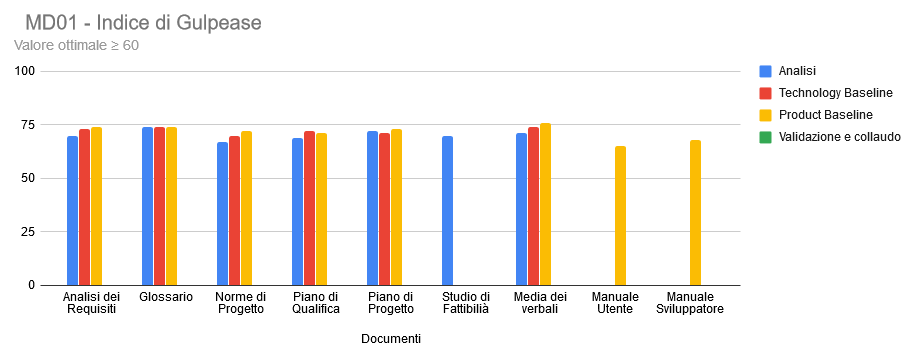
\includegraphics[scale=0.5]{./img/MD01_gulpease.png}
\caption{Grafico relativo ai dati di MD01 - Indice di Gulpease}
\end{figure}

\paragraph{Esiti Indice Fog} \mbox{} \\
\begin{longtable}{c c c c c c}
\rowcolor{white}\caption{Tabella Indice Fog} \\
		\rowcolor{redafk}
\textcolor{white}{\textbf{Attività}} &
\textcolor{white}{\textbf{An}} &
\textcolor{white}{\textbf{TB}} &
\textcolor{white}{\textbf{PB}} &
\textcolor{white}{\textbf{VC}} &
\textcolor{white}{\textbf{Riscontro}}  \\
		\endfirsthead
		\rowcolor{white}\caption[]{(continua)} \\
		\rowcolor{redafk}
\textcolor{white}{\textbf{Attività}} &
\textcolor{white}{\textbf{An}} &
\textcolor{white}{\textbf{TB}} &
\textcolor{white}{\textbf{PB}} &
\textcolor{white}{\textbf{VC}} &
\textcolor{white}{\textbf{Riscontro}}  \\
		\endhead
\textit{Analisi dei Requisiti} & 18 & 17 & - & - & Accettabile\\
\textit{Glossario} & 15 & 15 & - & - & Accettabile \\
\textit{Norme di Progetto} & 20 & 18 & - & - & Accettabile\\
\textit{Piano di Progetto} & 18 & 20 & - & - & Accettabile\\
\textit{Piano di Qualifica} & 20 & 20 & - & - & Accettabile\\
\textit{Studio di Fattibilità} & 14 & - & & & Accettabile\\
\textit{Media Verbali} & 8 & 6 & - & - & Ottimale\\
\end{longtable}

\begin{figure}[H]
\centering
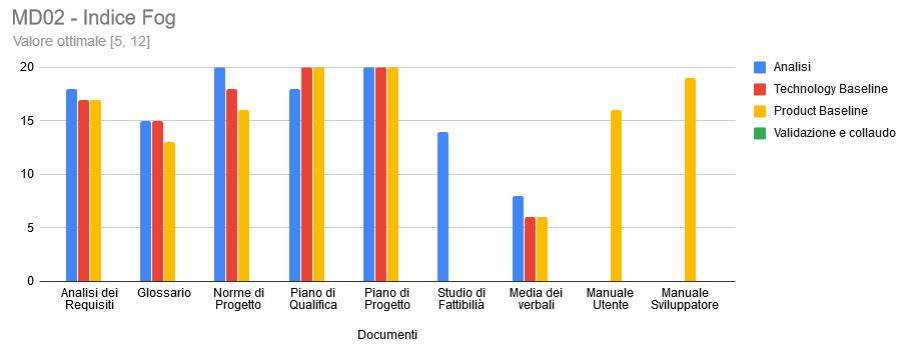
\includegraphics[scale=0.5]{./img/MD02_fog.png}
\caption{Grafico relativo ai dati di MD02 - Indice Fog}
\end{figure}

\subsection{Analisi dei processi}
\subsubsection{Esiti MP01 - Schedule Variance} 
\begin{longtable}{c c c c c c}
\rowcolor{white}\caption{Esiti verifica Schedule Variance} \\
		\rowcolor{redafk}
\textcolor{white}{\textbf{Attività}} &
\textcolor{white}{\textbf{An}} &
\textcolor{white}{\textbf{TB}} &
\textcolor{white}{\textbf{PB}} &
\textcolor{white}{\textbf{VC}} &
\textcolor{white}{\textbf{Riscontro}} \\
		\endfirsthead
		\rowcolor{white}\caption[]{(continua)} \\
		\rowcolor{redafk}
\textcolor{white}{\textbf{Attività}} &
\textcolor{white}{\textbf{An}} &
\textcolor{white}{\textbf{TB}} &
\textcolor{white}{\textbf{PB}} &
\textcolor{white}{\textbf{VC}} &
\textcolor{white}{\textbf{Riscontro}} \\
		\endhead
\textit{Analisi dei Requisiti} & 
1 &
4 &
- &
- &
Accettabile \\
\textit{Glossario} & 
0 &
0 &
- &
- &
Ottimale \\
\textit{Norme di Progetto} & 
0 &
5 &
- &
- &
Accettabile \\
\textit{Piano di Qualifica} & 
1 &
-2 &
- &
- &
Ottimale \\
\textit{Piano di Progetto} & 
1 &
0 &
- &
- &
Ottimale \\
\textit{Studio di Fattibilià} & 
0 &
- &
- &
- &
Ottimale \\
\end{longtable}

\begin{figure}[H]
\centering
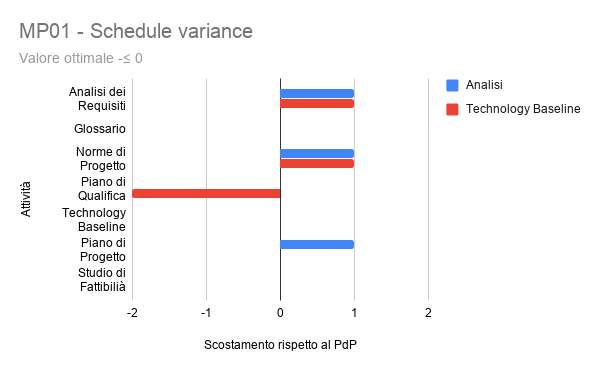
\includegraphics[scale=0.5]{./img/MP01_schedule_variance.png}
\caption{Grafico relativo ai dati di MP01 - Schedule Variance}
\end{figure}

\subsubsection{Esiti MP02 - Budget Variance}
\begin{longtable}{c c c c c}
\rowcolor{white}\caption{Esiti Budget Variance} \\
		\rowcolor{redafk}
\textcolor{white}{\textbf{An}} &
\textcolor{white}{\textbf{TB}} &
\textcolor{white}{\textbf{PB}} &
\textcolor{white}{\textbf{VC}} &
\textcolor{white}{\textbf{Riscontro}} \\
-8,66$\%$ &
-1,19$\%$ &
- &
- &
Accettabile \\
\end{longtable}

\begin{figure}[H]
\centering
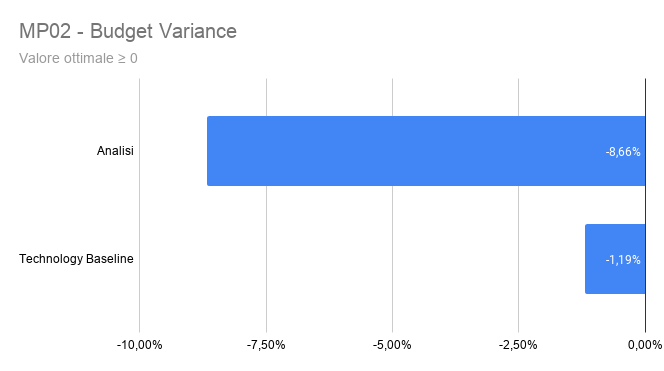
\includegraphics[scale=0.5]{./img/MP02_budget_variance.png}
\caption{Grafico relativo ai dati di MP02 - Budget Variance}
\end{figure}

\subsubsection{Esiti MP03 - Produttività} 
\begin{longtable}{c c c c c c}
\rowcolor{white}\caption{Esiti della Produttività} \\
		\rowcolor{redafk}
\textcolor{white}{\textbf{Membro}} &
\textcolor{white}{\textbf{An}} &
\textcolor{white}{\textbf{TB}} &
\textcolor{white}{\textbf{PB}} &
\textcolor{white}{\textbf{VC}} &
\textcolor{white}{\textbf{Riscontro}} \\
		\endfirsthead
		\rowcolor{white}\caption[]{(continua)} \\
		\rowcolor{redafk}
		\textcolor{white}{\textbf{Membro}} &
\textcolor{white}{\textbf{An}} &
\textcolor{white}{\textbf{TB}} &
\textcolor{white}{\textbf{PB}} &
\textcolor{white}{\textbf{VC}} &
\textcolor{white}{\textbf{Riscontro}} \\
		\endhead
Simone Federico Bergamin & 0 & 78 & - & - & Accettabile\\
Alessandro Canesso & 0 & 139 & - & - & Ottimale \\
Victor Dutca & 0 & 108 & - & - & Ottimale \\
Fouad Farid & 0 & 109 & - & - & Ottimale \\
Simone Meneghin & 0 & 93 & - & - & Accettabile\\
Olivier Utshudi & 0 & 93 & - & - & Accettabile\\
Davide Zillio & 0 & 93 & - & - & Accettabile

\begin{comment}
Metterei una nota a pié di pagina per spiegare che i valori sono a consuntivo e per questo, non sono alcuni componenti hanno scritto codice che in realtà non dovevano
\end{comment}
\end{longtable}


\begin{figure}[H]
\centering
\includegraphics[scale=0.5]{./img/MP03_produttività.png}
\caption{Grafico relativo ai dati di MP03 - Produttività}
\end{figure}
\pagebreak

\section{Valutazioni per il miglioramento}
In questa sezione viene riportata la valutazione fatta dal gruppo riguardo il lavoro svolto finora.
Lo scopo di questa scelta è trattare i problemi sorti e procedere alla loro più efficiente risoluzione
in modo tale che non si verifichino in futuro. \\
Verrano dunque tracciati problemi riguardanti i seguenti ambiti: \begin{itemize}
\item \textbf{Organizzazione}: vengono analizzati i problemi riguardanti l'organizzazione e la comunicazione all'interno del gruppo;
\item \textbf{Ruoli}: vengono analizzati i problemi riguardanti il corretto svolgimento di un ruolo;
\item \textbf{Strumenti di lavoro}: vengono analizzati i problemi riguardanti l'uso degli strumenti scelti.
\end{itemize}
Poichè non vi è una persona esterna che possa dare una valutazione oggettiva, ogni problema viene sollevato sulla base dell'autovalutazione dei soli membri del gruppo. Nonostante sia un sistema poco efficace, il gruppo ha beneficiato di questa scelta dal punto di vista comunicativo e produttivo, migliorando progressivamente la qualità del lavoro.\\
Questa sezione verrà aggiornata con l'avanzamento del prodotto riportando nuove problematiche, qualora queste dovessero verificarsi.

\subsection{Valutazioni sull'organizzazione}
\subsubsection{RR}
\begin{table}[H]
\caption{Problematiche relative all'organizzazione durante il periodo di RR}
\begin{center}
\begin{tabular}{ C{2.5cm} L{5cm} c L{5.5cm} }
\rowcolor{redafk}
\textcolor{white}{\textbf{Problema}} & \centerline{\textcolor{white}{\textbf{Descrizione}}} & \textcolor{white}{\textbf{Gravità}} & \centerline{\textcolor{white}{\textbf{Soluzione}}}\\
Incontro tra stakeholders\glo & A causa del Covid19, gli stakeholders hanno dovuto adattarsi alle restrizioni imposte, e tuttora in corso, impiegando tecnologie di comunicazione adatte allo smart working. & Bassa & Gli stakeholders hanno quindi utilizzato le tecnologie di comunicazione riportate nelle \textit{Norme di Progetto} per proseguire il progetto senza ulteriori intoppi. \\
\end{tabular}
\end{center}
\end{table}

\paragraph*{Considerazioni}\mbox{} \\ \mbox{} \\
In relazione al ciclo di Deming\glo si possono fare alcune considerazioni riguardo l'organizzazione del team.
Infatti l'obbiettivo (plan) è quello di individuare gli strumenti necessari a raggiungere una comunicazione fluida con gli stackeholders. Per raggiungere tale obiettivo sono state necessarie alcune prove (do), per via dei diversi mezzi di comunicazione a nostra disposizione. Infine sono stati scelti (act) gli opportuni mezzi sulla base dei riscontri (check) dei membri.

\subsubsection{RQ}
\begin{table}[H]
\caption{Problematiche relative all'organizzazione durante il periodo di RQ}
\begin{center}
\begin{tabular}{ C{2.5cm} L{5cm} c L{5.5cm} }
\rowcolor{redafk}
\textcolor{white}{\textbf{Problema}} & \centerline{\textcolor{white}{\textbf{Descrizione}}} & \textcolor{white}{\textbf{Gravità}} & \centerline{\textcolor{white}{\textbf{Soluzione}}}\\
Gestione del tempo a disposizione & A causa dei vari esami arretrati da parte di alcuni componenti del team, è risultato difficile gestire il tempo a dispozione in modo ottimale per proseguire il progetto senza intoppi. & Alta & Il \textit{Responsabile di Progetto} ha suddiviso nuovamente i vari task da svolgere in base alle possibilità di ogni componente. È stato quindi deciso di affidare ai membri più impegnati i compiti meno complicati, per permettere lo svolgimento del progetto in modo collaborativo e parallelo.
\end{tabular}
\end{center}
\end{table}

\paragraph*{Considerazioni}\mbox{} \\ \mbox{} \\
Il \textit{Responsabile di Progetto} ha avuto ruolo chiave nella risoluzione di questo problema. La soluzione adottata infatti ha permesso di proseguire lo sviluppo del progetto (documenti e software) senza rallentamenti. Il \textit{TeamAFK} ha già preso in considerazione la possibilità che questo problema possa ripresentarsi durante la Revisione di Accettazione.
\pagebreak
\subsection{Valutazioni sui ruoli}
\subsubsection{RR}
\begin{table}[H]
\caption{Problematiche relative ai ruoli riscontrati durante la RR}
\begin{center}
\begin{tabular}{ C{2.5cm} L{5cm} c L{5.5cm} }
\rowcolor{redafk}
\textcolor{white}{\textbf{Problema}} & \centerline{\textcolor{white}{\textbf{Descrizione}}} & \textcolor{white}{\textbf{Gravità}} & \centerline{\textcolor{white}{\textbf{Soluzione}}}\\
Ruolo di \textit{Responsabile} & A causa dell'inesperienza, chi ha lavorato come \textit{Responsabile} ha avuto difficoltà nella suddivisione bilanciata delle ore tra i membri provocando diverse ridistribuzioni delle ore. & Alta & Per evitare eventuali ritardi nelle consegne, il gruppo ha deciso di dedicare del tempo per analizzare meglio la mole di lavoro e compiere così una più accurata distribuzione delle ore. \\
\end{tabular}
\end{center}
\end{table}

\paragraph*{Considerazioni}\mbox{} \\ \mbox{} \\
Per via dell'inesperienza del team non è stato possibile stabilire  il miglior approccio nella gestione del tempo e per questo sono emerse alcune difficolte per alcuni ruoli. Nonostante ciò tramite le segnalazioni dei membri (check), è possibile comprendere e risolvere le problematiche adottando anche differenti approcci. Il tutto per ottimizzare il tempo messo a disposizione per ciascun componente e quindi rispettare le scadenze (plan).

\subsubsection{RP}
\begin{table}[H]
\caption{Problematiche relative ai ruoli riscontrati durante la RP}
\begin{center}
\begin{tabular}{ C{2.5cm} L{5cm} c L{5.5cm} }
\rowcolor{redafk}
\textcolor{white}{\textbf{Problema}} & \centerline{\textcolor{white}{\textbf{Descrizione}}} & \textcolor{white}{\textbf{Gravità}} & \centerline{\textcolor{white}{\textbf{Soluzione}}}\\
Ruolo di \textit{Progettista} & L’attività di progettazione è stata molto complessa e abbiamo riscontrato più difficoltà di quanto preventivato. & Alta & Si è deciso di assegnare più ore ai progettisti a scapito di altri ruoli per riuscire a comprendere e realizzare una buona architettura del nostro prodotto. \\
\end{tabular}
\end{center}
\end{table}
\paragraph*{Considerazioni}\mbox{} \\ \mbox{} \\
La soluzione adottata ha migliorato la situazione e ha permesso di svolgere il lavoro pianificato rispettando tempi e budget.
\pagebreak
\subsection{Valutazioni sugli strumenti di lavoro}
\subsubsection{RR}
\begin{longtable}{ C{2.3cm} L{5.5cm} c L{5.5cm} }
\rowcolor{white}\caption{Problematiche relative agli strumenti di lavoro durante la RR}\\
		\rowcolor{redafk}
\textcolor{white}{\textbf{Problema}} & \centerline{\textcolor{white}{\textbf{Descrizione}}} & \textcolor{white}{\textbf{Gravità}} & \centerline{\textcolor{white}{\textbf{Soluzione}}}\\
		\endfirsthead
		\rowcolor{white}\caption[]{(continua)} \\
		\rowcolor{redafk}
\textcolor{white}{\textbf{Problema}} & \centerline{\textcolor{white}{\textbf{Descrizione}}} & \textcolor{white}{\textbf{Gravità}} & \centerline{\textcolor{white}{\textbf{Soluzione}}}\\
		\endhead
GitHub & Si sono riscontrati in più occasioni
conflitti sui file in cui si stava lavorando e il tempo utilizzato per risolverli è stato sottratto dal tempo di lavoro. & Media & Il gruppo è stato istruito sull’uso di specifici branch\glo in modo tale che la modifiche di tutti i componenti si potessero integrare con il proprio lavoro senza che quest’ultimo potesse avere dei conflitti. \\
\LaTeX{} & A causa dell’inesperienza di
alcuni membri del gruppo nell’utilizzo
di questo strumento, si sono riscontrate diverse
difficoltà sopratutto nella costruzione di tabelle e nell'inserimento di formule matematiche. & Bassa & Per risolvere in breve tempo questa problematica, si è deciso di affiancare ai membri meno esperti chi sapeva già utilizzare i comandi di \LaTeX{} dando così la possibilità ai primi di imparare e permettendo ai secondi di non subire grossi rallentamenti nel lavoro. \\
\end{longtable}

\subsubsection{RP}
\begin{longtable}{ C{2.3cm} L{5.5cm} c L{5.5cm} }
\rowcolor{white}\caption{Problematiche relative agli strumenti di lavoro durante la RP}\\
		\rowcolor{redafk}
\textcolor{white}{\textbf{Problema}} & \centerline{\textcolor{white}{\textbf{Descrizione}}} & \textcolor{white}{\textbf{Gravità}} & \centerline{\textcolor{white}{\textbf{Soluzione}}}\\
		\endfirsthead
		\rowcolor{white}\caption[]{(continua)} \\
		\rowcolor{redafk}
\textcolor{white}{\textbf{Problema}} & \centerline{\textcolor{white}{\textbf{Descrizione}}} & \textcolor{white}{\textbf{Gravità}} & \centerline{\textcolor{white}{\textbf{Soluzione}}}\\
		\endhead
IntelliJ & A causa dell’inesperienza di alcuni membri del gruppo nell’utilizzo
di questo IDE, si sono riscontrate alcune difficoltà nell'apprendimento delle funzionalità necessarie per lo sviluppo del software. & Bassa & Per risolvere in breve tempo questa problematica, si è deciso di affiancare ai membri meno esperti chi sapeva già utilizzare questo strumento. \\
NPM & Si sono riscontrate delle problematiche durante la fase di configurazione di questo strumento, dovute soprattutto all'installazione di quest'ultimo in diversi sistemi operativi (Windows, Linux). & Media & Il \textit{TeamAFK} ha deciso di installare una versione stabile comune di questo strumento nei sistemi operativi in uso, evitando problemi di integrazione.
\end{longtable}

\pagebreak
\subsection{Valutazione globale}

\subsubsection{Analisi}
La prima critica costruttiva che ci poniamo riguarda il periodo di analisi.
Durante la prima parte del progetto, che dovrebbe essere dedicata maggiormente
all’analisi e alla definizione dei requisiti del nostro prodotto, non
ci siamo soffermati a sufficienza per comprenderli fino in fondo. Perciò, nei
periodi successivi, abbiamo dovuto spendere più ore nel ruolo di analista, riducendo
di conseguenza il numero di ore dedicate ad altri ruoli che avrebbero
potuto portare allo sviluppo di funzionalità aggiuntive.

\subsubsection{Sviluppo ed implementazione dei test}
La seconda critica costruttiva che ci poniamo riguarda lo sviluppo ed implementazione dei test, in modo particolare i test di unità. Quest'ultimi sono risultati non banali da sviluppare ed inizialmente ci siamo posti l’obiettivo di implementare più test possibili, indistintamente dalla loro priorità. In questo modo abbiamo impiegato un numero importante di ore nel ruolo di verificatore mentre se avessimo implementato i test con più raziocinio, avremmo avuto più ore da impiegare in altri ruoli, quali progettista e programmatore, per sviluppare funzionalità aggiuntive o raffinare alcuni dettagli.

\subsubsection{Valutazione per il miglioramento}
L'alternativa più efficace al nostro processo di miglioramento continuo sarebbe stata l’implementazione del ciclo di Deming: plan - do - check - act. Consiste nella
pianificazione dell’azione migliorativa (plan), nel monitoraggio della sua esecuzione
(do), nella verifica del suo esito (check) e nella valutazione critica
della sua efficacia (act) che può portare ad un’approvazione o, in caso di
insuccesso, ad un’ulteriore ripetizione del ciclo. Seguendo questo approccio,
avremmo potuto identificare le possibili migliorie da apportare in modo più
efficace e più dettagliato.

\subsubsection{Conclusioni}
Le metriche di qualità che ci siamo posti inizialmente sono state soddisfatte
con valori di accettabilità e spesso anche di ottimalità quindi siamo soddisfatti del nostro lavoro. Abbiamo avuto dei riscontri sempre più positivi da parte del committente e del proponente, e proprio quest’ultimo, durante uno degli ultimi incontri, si è detto soddisfatto del prodotto che abbiamo sviluppato.
\pagebreak


\end{document}